\begin{flushleft}
    Wie in unserer Evaluation der Lösungsideen bereits beschrieben übernimmt der ESP32 Microcontroller, siehe Abbildung \ref{fig:esp32_mc}, die Steuerung unseres Roboters. 
    
    \begin{figure}[h!]
        \centering
        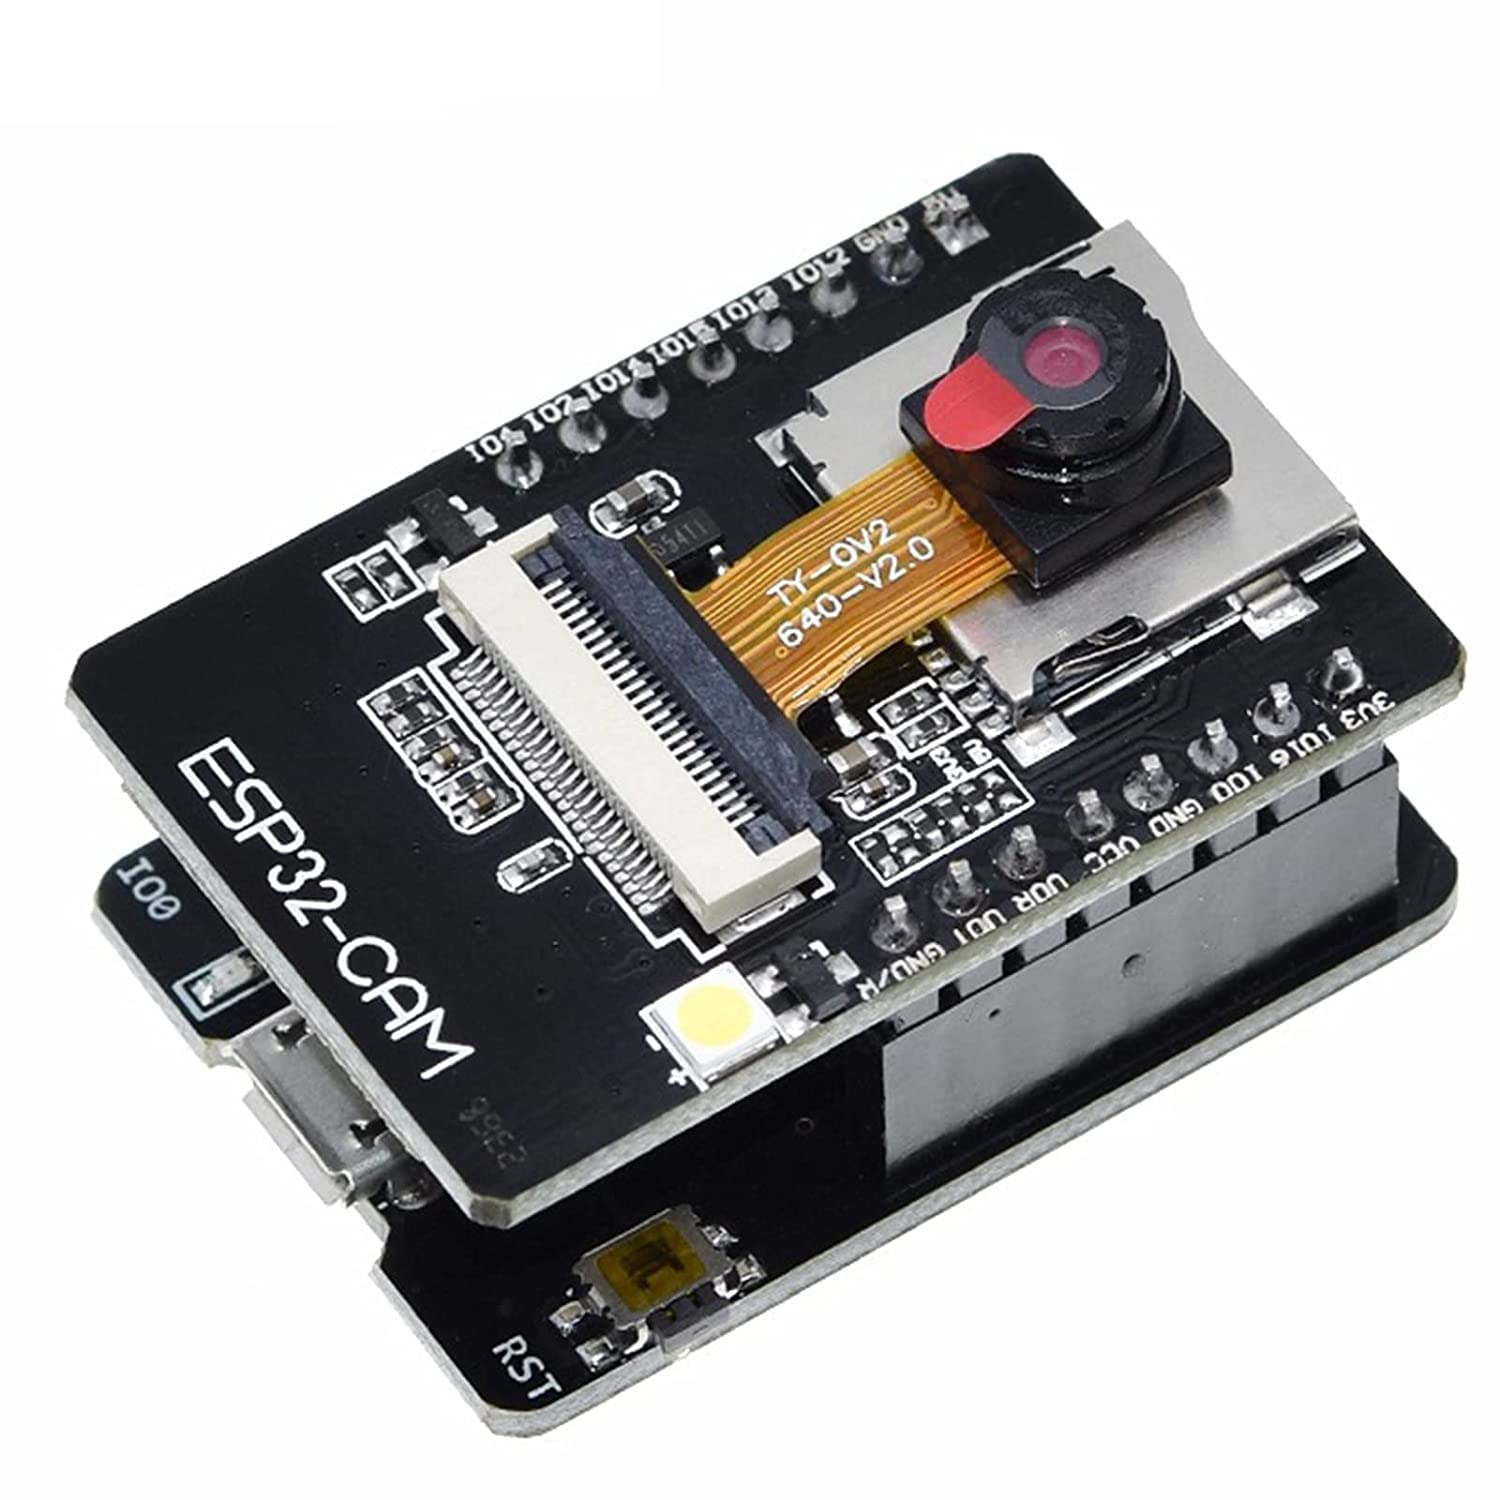
\includegraphics[width=0.3\textwidth]{imgs/Roboter/Real/esp32.jpg}
        \caption{ESP32 Microcontroller}
        \label{fig:esp32_mc}%
    \end{figure}

    Dieser muss natürlich auch mit Spannung versogt werden.
    Der Akku unseres Roboter sind sogenannte 18650 LiIon Akkus, diese sind wiederaufladbar und haben die perfekte Größe 
    für unseren kleinen Roboter.

    Die Versorgungsspannung für die Motoren kann direkt von unserem Akkupack abgegriffen werden und zur H-Brücke geführt werden.
    Die H-Brücke benötigt genau so wie der ESP32 eine Versorgungsspannung für die Logik.
    Diese sollte laut Datenblatt bei 5V liegen, erlaubt sind aber auch 3V. Was in unserem Fall ideal ist da unser ESP32
    ebenfalls nur mit 3,3V maxmimal versorgt werden darf.

    Die 3,3V Logikspannung werden auf unserer Platine von einem LM317T, einem Lineareren Spannungswandler zur Verfügung gestellt.

    \begin{figure}[h!]
        \centering
        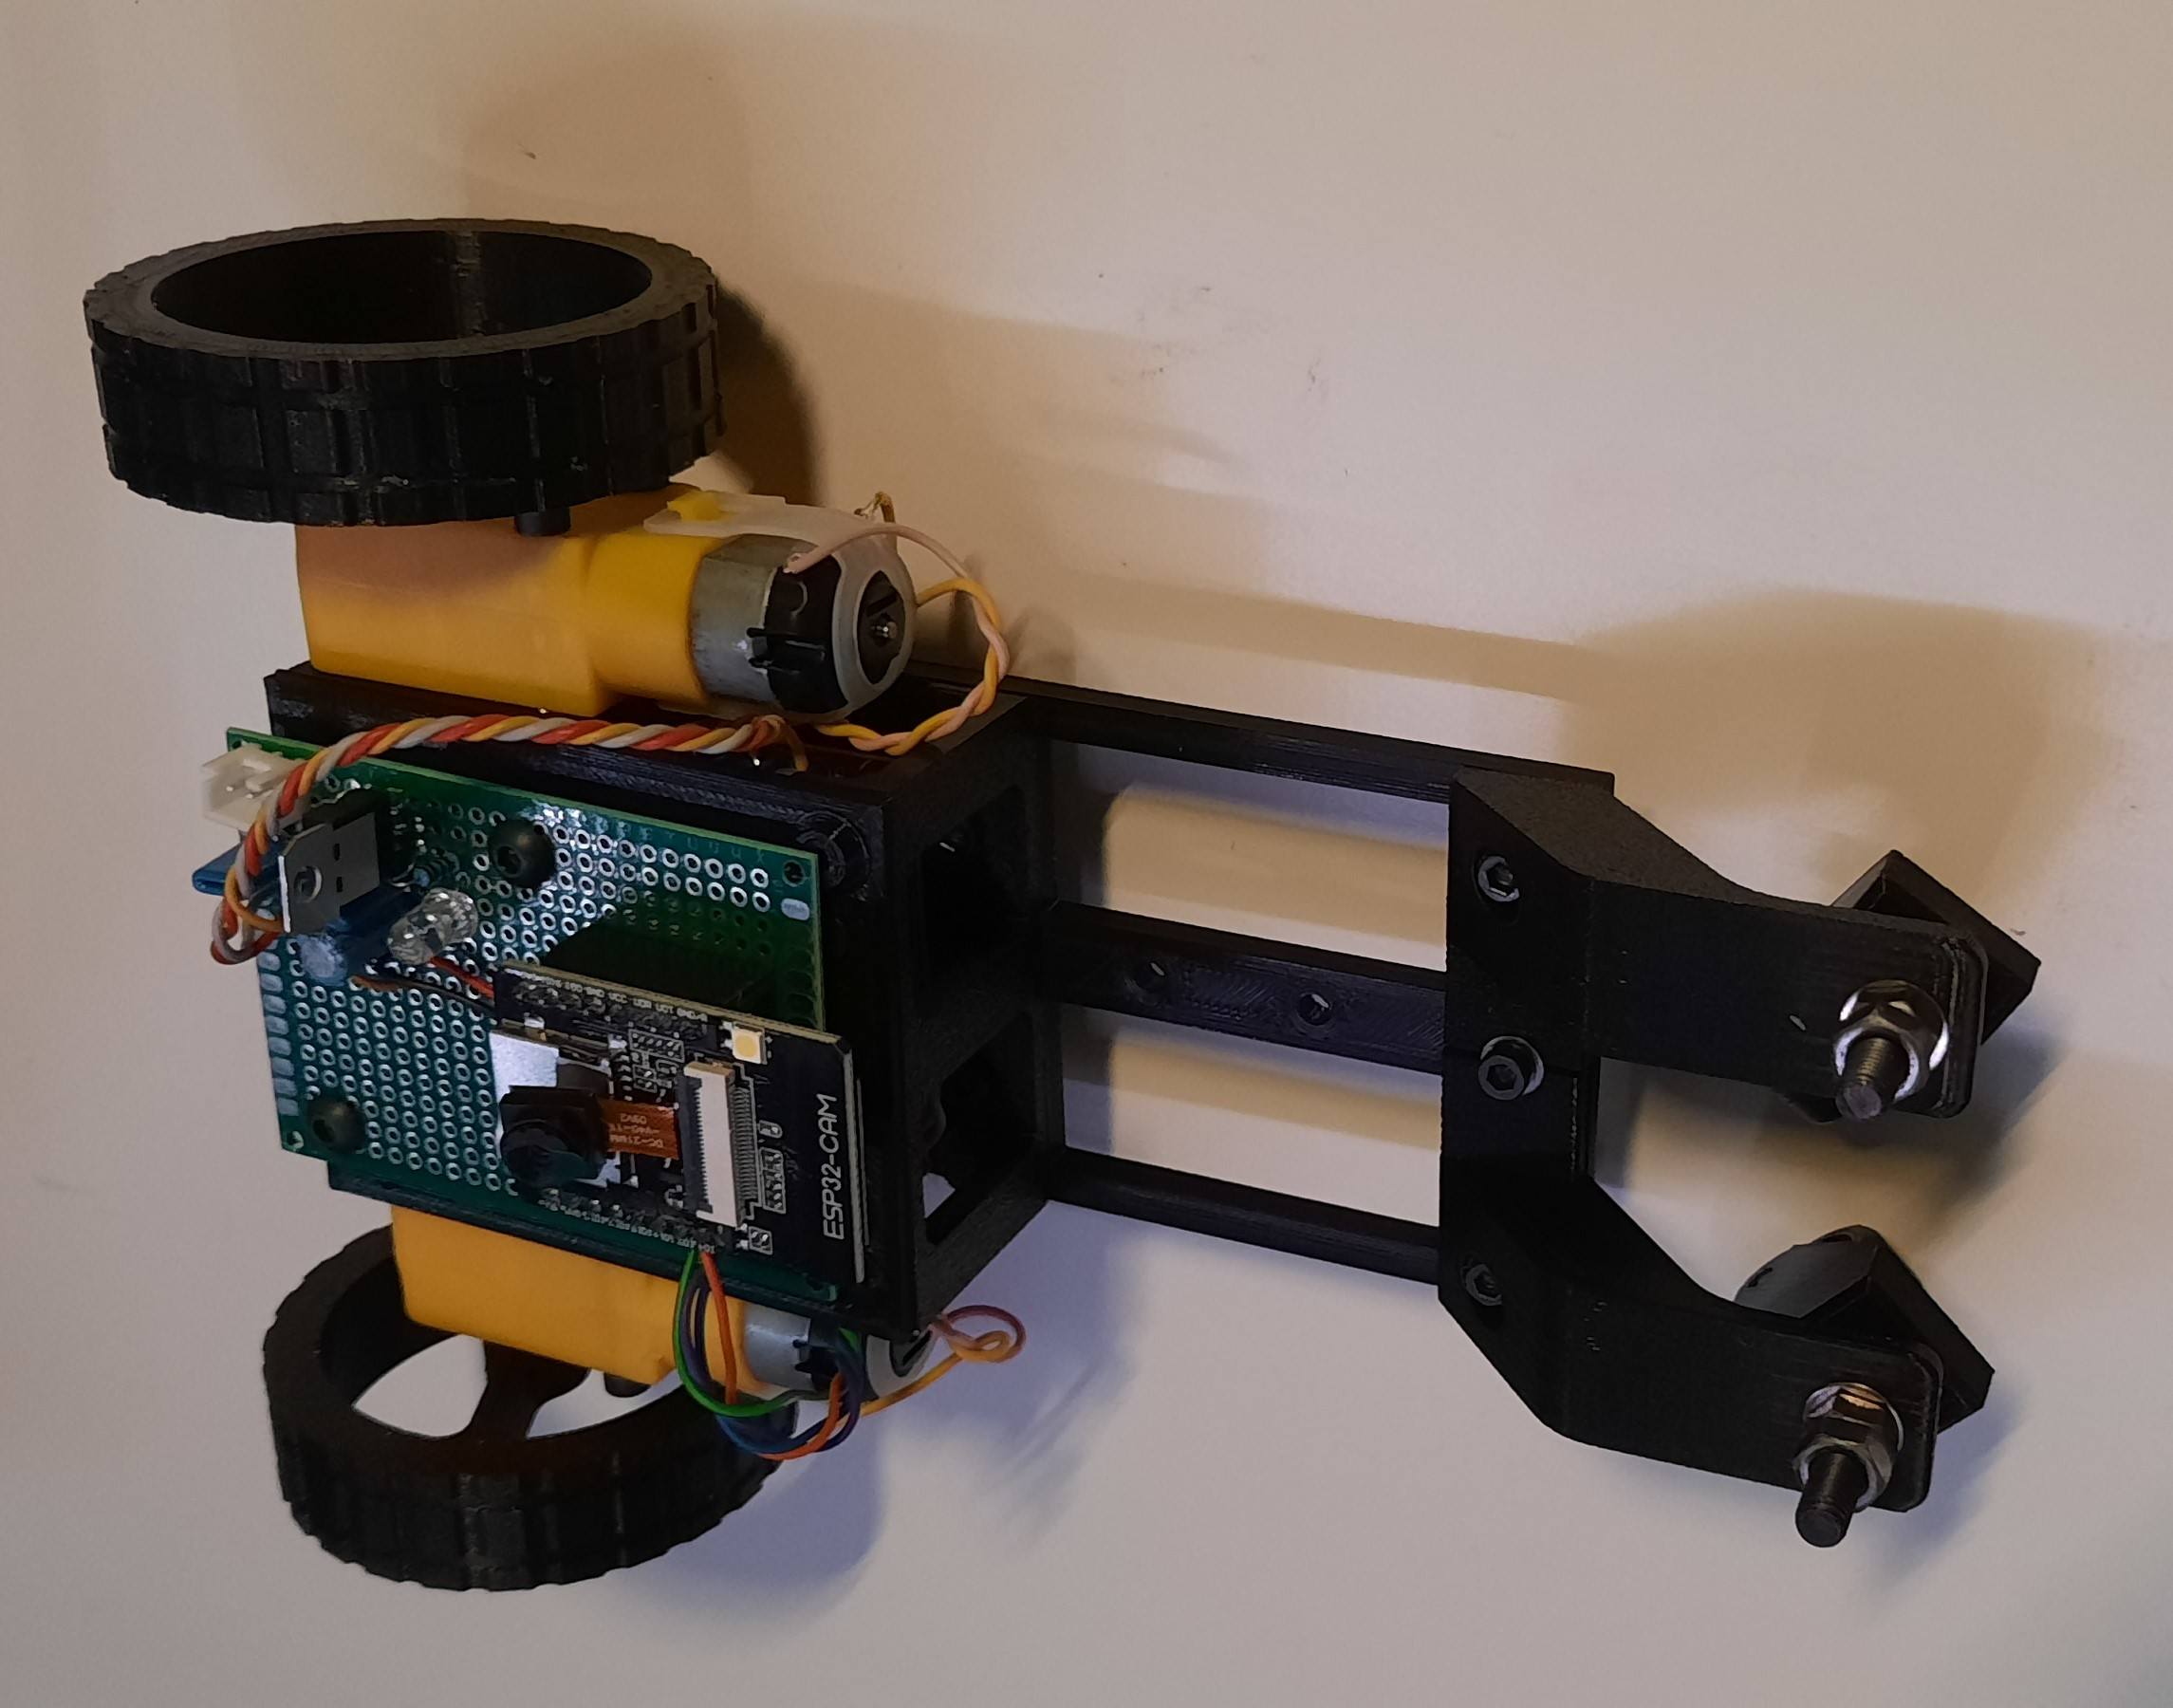
\includegraphics[width=0.5\textwidth, angle=-90,origin=c]{imgs/Roboter/Real/Roboter.jpg}
        \caption{Roboter Demo Platform}
      \end{figure}

\end{flushleft}